\documentclass[border=4pt]{standalone}
% Preámbulo común de las figuras. Cada figura es un documento standalone
% que se compila a SVG con scripts/build_figures.sh
\usepackage[utf8]{inputenc}
\usepackage{amsmath}
\usepackage{tikz}
\usepackage[american, siunitx]{circuitikz}
\usetikzlibrary{arrows.meta,calc,decorations.pathmorphing,patterns}
\tikzset{
  >={Stealth[length=2.2mm]},
  eje/.style={->, thin},
  hilo/.style={thick},
}
% Paleta común: tonos medios legibles sobre fondo claro
\definecolor{azul}{RGB}{31,94,168}
\definecolor{rojo}{RGB}{192,57,43}
\definecolor{verde}{RGB}{39,128,73}
\definecolor{naranja}{RGB}{211,120,30}
\definecolor{morado}{RGB}{125,60,152}

\begin{document}
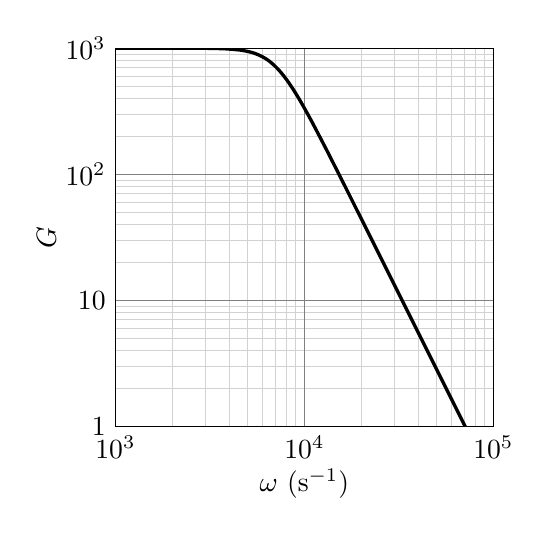
\begin{tikzpicture}[x=2.4cm, y=1.6cm]
  % ejes log-log: x = log10(omega) - 3, y = log10(G)
  \foreach \d in {0,1} {
    \foreach \k in {2,...,9} \draw[gray!35, very thin] ({\d+log10(\k)},0) -- ({\d+log10(\k)},3);
  }
  \foreach \d in {0,1,2} {
    \foreach \k in {2,...,9} \draw[gray!35, very thin] (0,{\d+log10(\k)}) -- (2,{\d+log10(\k)});
  }
  \foreach \x in {0,1,2} \draw[gray] (\x,0) -- (\x,3);
  \foreach \y in {0,1,2,3} \draw[gray] (0,\y) -- (2,\y);
  \draw (0,0) rectangle (2,3);
  \node[below] at (0,0) {$10^{3}$};
  \node[below] at (1,0) {$10^{4}$};
  \node[below] at (2,0) {$10^{5}$};
  \node[left] at (0,0) {$1$};
  \node[left] at (0,1) {$10$};
  \node[left] at (0,2) {$10^{2}$};
  \node[left] at (0,3) {$10^{3}$};
  \node[below=12pt] at (1,0) {$\omega$ (s$^{-1}$)};
  \node[rotate=90, above=18pt] at (0,1.5) {$G$};
  \clip (0,0) rectangle (2,3);
  \draw[very thick] plot[smooth] coordinates {(0.00,3.000) (0.02,3.000) (0.04,3.000) (0.06,3.000) (0.08,3.000) (0.10,3.000) (0.12,3.000) (0.14,3.000) (0.16,3.000) (0.18,3.000) (0.20,3.000) (0.22,3.000) (0.24,3.000) (0.26,3.000) (0.28,3.000) (0.30,3.000) (0.32,3.000) (0.34,3.000) (0.36,3.000) (0.38,3.000) (0.40,3.000) (0.42,2.999) (0.44,2.999) (0.46,2.999) (0.48,2.999) (0.50,2.998) (0.52,2.998) (0.54,2.997) (0.56,2.996) (0.58,2.995) (0.60,2.993) (0.62,2.991) (0.64,2.988) (0.66,2.985) (0.68,2.980) (0.70,2.974) (0.72,2.967) (0.74,2.957) (0.76,2.945) (0.78,2.930) (0.80,2.912) (0.82,2.890) (0.84,2.864) (0.86,2.834) (0.88,2.800) (0.90,2.762) (0.92,2.720) (0.94,2.675) (0.96,2.627) (0.98,2.577) (1.00,2.524) (1.02,2.470) (1.04,2.415) (1.06,2.358) (1.08,2.301) (1.10,2.243) (1.12,2.185) (1.14,2.126) (1.16,2.067) (1.18,2.008) (1.20,1.948) (1.22,1.889) (1.24,1.829) (1.26,1.769) (1.28,1.709) (1.30,1.650) (1.32,1.590) (1.34,1.530) (1.36,1.470) (1.38,1.410) (1.40,1.350) (1.42,1.290) (1.44,1.230) (1.46,1.170) (1.48,1.110) (1.50,1.050) (1.52,0.990) (1.54,0.930) (1.56,0.870) (1.58,0.810) (1.60,0.750) (1.62,0.690) (1.64,0.630) (1.66,0.570) (1.68,0.510) (1.70,0.450) (1.72,0.390) (1.74,0.330) (1.76,0.270) (1.78,0.210) (1.80,0.150) (1.82,0.090) (1.84,0.030) (1.86,-0.030) (1.88,-0.090) (1.90,-0.150) (1.92,-0.210) (1.94,-0.270) (1.96,-0.330) (1.98,-0.390) (2.00,-0.450)};
\end{tikzpicture}
\end{document}
